% Options for packages loaded elsewhere
\PassOptionsToPackage{unicode}{hyperref}
\PassOptionsToPackage{hyphens}{url}
%
\documentclass[
]{book}
\usepackage{amsmath,amssymb}
\usepackage{lmodern}
\usepackage{iftex}
\ifPDFTeX
  \usepackage[T1]{fontenc}
  \usepackage[utf8]{inputenc}
  \usepackage{textcomp} % provide euro and other symbols
\else % if luatex or xetex
  \usepackage{unicode-math}
  \defaultfontfeatures{Scale=MatchLowercase}
  \defaultfontfeatures[\rmfamily]{Ligatures=TeX,Scale=1}
\fi
% Use upquote if available, for straight quotes in verbatim environments
\IfFileExists{upquote.sty}{\usepackage{upquote}}{}
\IfFileExists{microtype.sty}{% use microtype if available
  \usepackage[]{microtype}
  \UseMicrotypeSet[protrusion]{basicmath} % disable protrusion for tt fonts
}{}
\makeatletter
\@ifundefined{KOMAClassName}{% if non-KOMA class
  \IfFileExists{parskip.sty}{%
    \usepackage{parskip}
  }{% else
    \setlength{\parindent}{0pt}
    \setlength{\parskip}{6pt plus 2pt minus 1pt}}
}{% if KOMA class
  \KOMAoptions{parskip=half}}
\makeatother
\usepackage{xcolor}
\usepackage{longtable,booktabs,array}
\usepackage{calc} % for calculating minipage widths
% Correct order of tables after \paragraph or \subparagraph
\usepackage{etoolbox}
\makeatletter
\patchcmd\longtable{\par}{\if@noskipsec\mbox{}\fi\par}{}{}
\makeatother
% Allow footnotes in longtable head/foot
\IfFileExists{footnotehyper.sty}{\usepackage{footnotehyper}}{\usepackage{footnote}}
\makesavenoteenv{longtable}
\usepackage{graphicx}
\makeatletter
\def\maxwidth{\ifdim\Gin@nat@width>\linewidth\linewidth\else\Gin@nat@width\fi}
\def\maxheight{\ifdim\Gin@nat@height>\textheight\textheight\else\Gin@nat@height\fi}
\makeatother
% Scale images if necessary, so that they will not overflow the page
% margins by default, and it is still possible to overwrite the defaults
% using explicit options in \includegraphics[width, height, ...]{}
\setkeys{Gin}{width=\maxwidth,height=\maxheight,keepaspectratio}
% Set default figure placement to htbp
\makeatletter
\def\fps@figure{htbp}
\makeatother
\setlength{\emergencystretch}{3em} % prevent overfull lines
\providecommand{\tightlist}{%
  \setlength{\itemsep}{0pt}\setlength{\parskip}{0pt}}
\setcounter{secnumdepth}{5}
\usepackage{booktabs}
\usepackage{booktabs}
\usepackage{longtable}
\usepackage{array}
\usepackage{multirow}
\usepackage{wrapfig}
\usepackage{float}
\usepackage{colortbl}
\usepackage{pdflscape}
\usepackage{tabu}
\usepackage{threeparttable}
\usepackage{threeparttablex}
\usepackage[normalem]{ulem}
\usepackage{makecell}
\usepackage{xcolor}
\ifLuaTeX
  \usepackage{selnolig}  % disable illegal ligatures
\fi
\usepackage[]{natbib}
\bibliographystyle{plainnat}
\IfFileExists{bookmark.sty}{\usepackage{bookmark}}{\usepackage{hyperref}}
\IfFileExists{xurl.sty}{\usepackage{xurl}}{} % add URL line breaks if available
\urlstyle{same} % disable monospaced font for URLs
\hypersetup{
  pdftitle={Streetlight and Transport Walking},
  pdfauthor={Tharindu Bandara},
  hidelinks,
  pdfcreator={LaTeX via pandoc}}

\title{Streetlight and Transport Walking}
\author{Tharindu Bandara}
\date{2024-03-07}

\begin{document}
\maketitle

{
\setcounter{tocdepth}{1}
\tableofcontents
}
\hypertarget{data-preparation}{%
\chapter{Data preparation}\label{data-preparation}}

The same steps followed as Gavin did for his 2014 paper (chapter 3).

\begin{itemize}
\tightlist
\item
  Excluded the participants who moved residence in between surveys
\item
  Excluded the respondents who were not the same person at each wave
\item
  Excluded the respondents who had missing values for transport walking for all waves
\item
  Excluded the participants who had missing values for education
\end{itemize}

\hypertarget{streetlight-count}{%
\chapter{Streetlight count}\label{streetlight-count}}

Streetlights is the built environment attribute of interest.

\begin{itemize}
\tightlist
\item
  Street light BE attribute is measured as 1km network buffer of residence.
\end{itemize}

\hypertarget{descriptives}{%
\section{Descriptives}\label{descriptives}}

\hypertarget{descriptive-statistics-of-streetlight-counts-at-each-wave.}{%
\subsection{Descriptive statistics of Streetlight counts at each wave.}\label{descriptive-statistics-of-streetlight-counts-at-each-wave.}}

\begin{table}
\centering\begingroup\fontsize{15}{17}\selectfont

\begin{tabular}{lrrrrr}
\toprule
\multicolumn{1}{c}{ } & \multicolumn{5}{c}{Streetlight summary} \\
\cmidrule(l{3pt}r{3pt}){2-6}
  & 2007 & 2009 & 2011 & 2013 & 2016\\
\midrule
Min. & 0.0000 & 0.0000 & 0.0000 & 0.0000 & 0.0000\\
1st Qu. & 172.0000 & 165.0000 & 200.0000 & 215.0000 & 214.0000\\
Median & 254.5000 & 252.0000 & 285.0000 & 296.0000 & 302.0000\\
Mean & 264.8033 & 254.7097 & 290.1867 & 302.0529 & 306.6352\\
3rd Qu. & 347.0000 & 349.0000 & 371.0000 & 382.0000 & 389.0000\\
\addlinespace
Max & 1159.0000 & 1170.0000 & 1226.0000 & 1232.0000 & 1264.0000\\
Missing & 0.0000 & 2760.0000 & 3637.0000 & 4002.0000 & 5078.0000\\
\bottomrule
\end{tabular}
\endgroup{}
\end{table}

\hypertarget{distribution}{%
\subsection{Distribution}\label{distribution}}

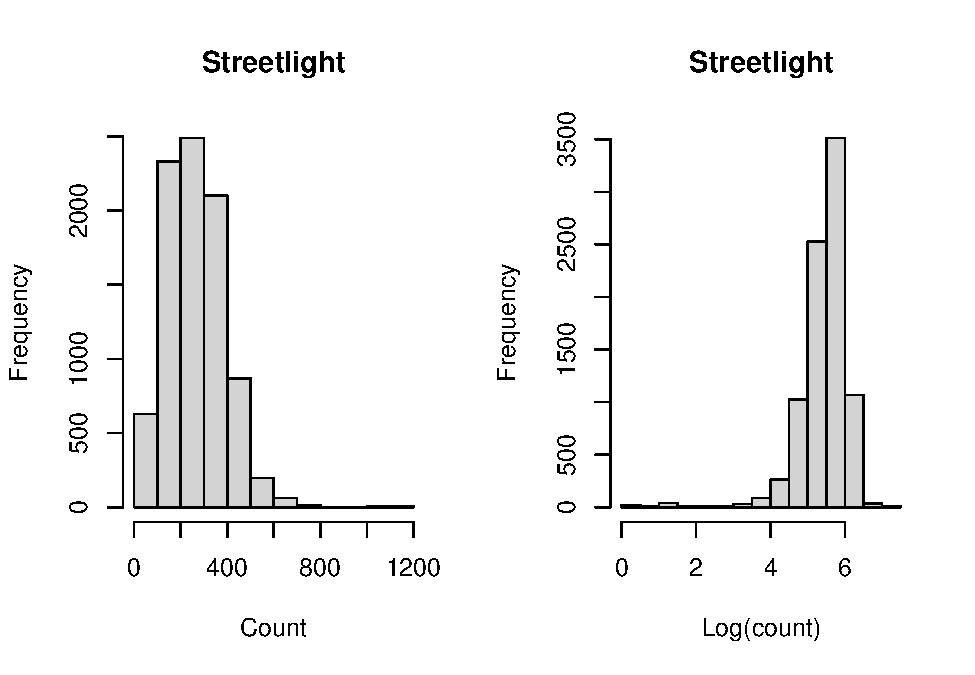
\includegraphics{_main_files/figure-latex/plots-1.pdf} 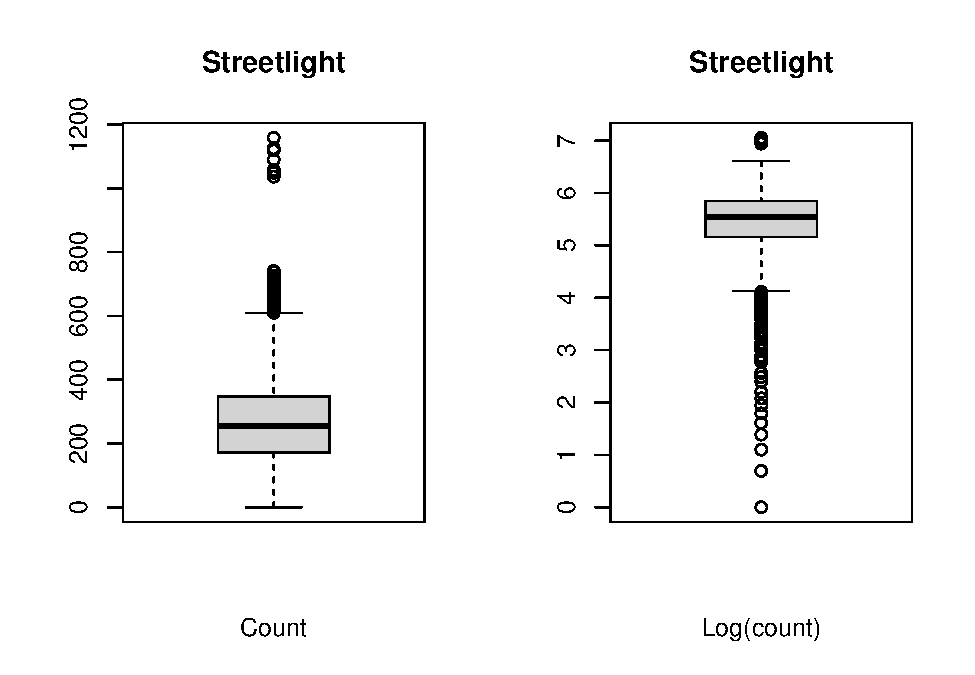
\includegraphics{_main_files/figure-latex/plots-2.pdf}

There were 13 participants having grater than 1000 streetlight counts, others have less than 800 streetlight counts.
Following plots are without these participants.
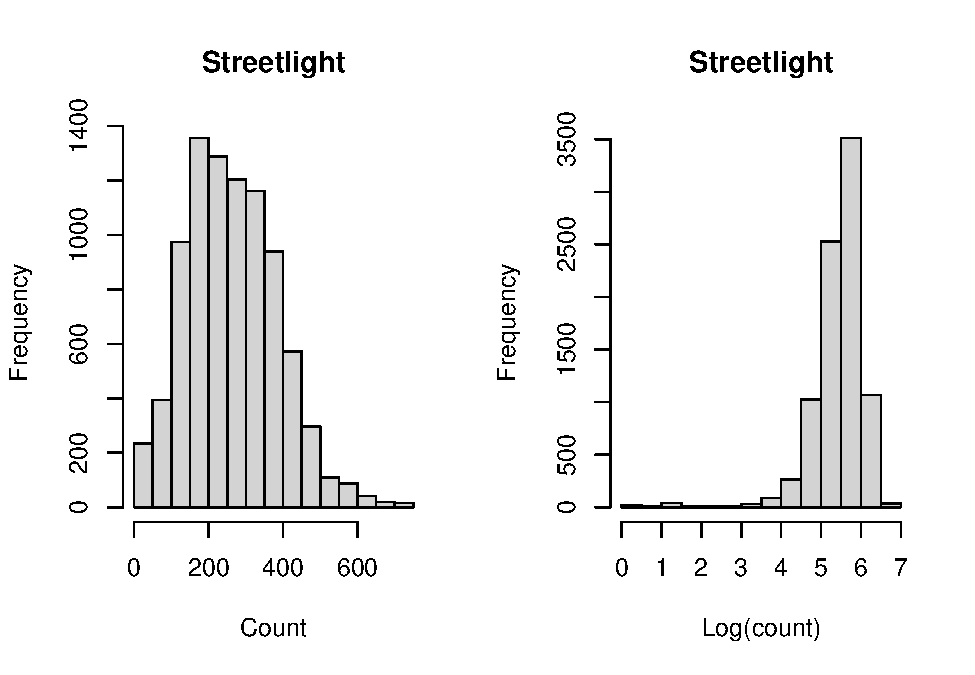
\includegraphics{_main_files/figure-latex/plots-w/o-outliers-1.pdf} 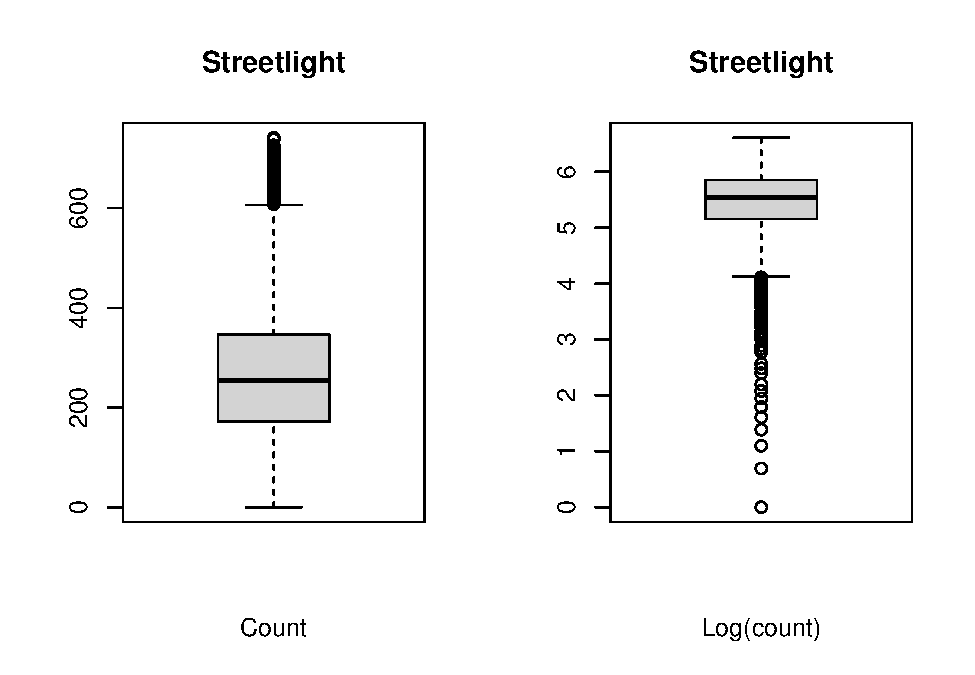
\includegraphics{_main_files/figure-latex/plots-w/o-outliers-2.pdf}

\hypertarget{one-way-anova-tests}{%
\section{One-way ANOVA tests}\label{one-way-anova-tests}}

\begin{verbatim}
##               Df    Sum Sq  Mean Sq F value Pr(>F)    
## habneigh1      1  39020790 39020790    3325 <2e-16 ***
## Residuals   8708 102180176    11734                   
## ---
## Signif. codes:  0 '***' 0.001 '**' 0.01 '*' 0.05 '.' 0.1 ' ' 1
\end{verbatim}

ANOVA test for Log transformed streetlight counts

\begin{verbatim}
##               Df Sum Sq Mean Sq F value Pr(>F)    
## habneigh1      1    731   730.6    1818 <2e-16 ***
## Residuals   8667   3483     0.4                   
## ---
## Signif. codes:  0 '***' 0.001 '**' 0.01 '*' 0.05 '.' 0.1 ' ' 1
\end{verbatim}

Following one-way ANOVA tests without the 13 records

\begin{verbatim}
##               Df   Sum Sq  Mean Sq F value Pr(>F)    
## habneigh1      1 36284234 36284234    3298 <2e-16 ***
## Residuals   8695 95650812    11001                   
## ---
## Signif. codes:  0 '***' 0.001 '**' 0.01 '*' 0.05 '.' 0.1 ' ' 1
\end{verbatim}

ANOVA test for Log transformed streetlight counts

\begin{verbatim}
##               Df Sum Sq Mean Sq F value Pr(>F)    
## habneigh1      1    711   710.7    1772 <2e-16 ***
## Residuals   8654   3471     0.4                   
## ---
## Signif. codes:  0 '***' 0.001 '**' 0.01 '*' 0.05 '.' 0.1 ' ' 1
\end{verbatim}

\hypertarget{sample-profile}{%
\chapter{Sample Profile}\label{sample-profile}}

Never walker is defined as participants who reportedly didn't walk for transport at each wave they responded to.

\begin{table}
\centering\begingroup\fontsize{15}{17}\selectfont

\begin{tabular}{lrrrrr}
\toprule
\multicolumn{1}{c}{ } & \multicolumn{5}{c}{Never-walkers} \\
\cmidrule(l{3pt}r{3pt}){2-6}
\multicolumn{1}{c}{ } & \multicolumn{1}{c}{2007} & \multicolumn{1}{c}{2009} & \multicolumn{1}{c}{2011} & \multicolumn{1}{c}{2013} & \multicolumn{1}{c}{2016} \\
\cmidrule(l{3pt}r{3pt}){2-2} \cmidrule(l{3pt}r{3pt}){3-3} \cmidrule(l{3pt}r{3pt}){4-4} \cmidrule(l{3pt}r{3pt}){5-5} \cmidrule(l{3pt}r{3pt}){6-6}
  & \% & \% & \% & \% & \%\\
\midrule
\addlinespace[0.3em]
\multicolumn{6}{l}{\textbf{Sex}}\\
\hspace{1em}Male & 63.7 & 60.8 & 60.4 & 58.7 & 55.1\\
\hspace{1em}Female & 66.7 & 63.2 & 64.1 & 64.1 & 60.5\\
\addlinespace[0.3em]
\multicolumn{6}{l}{\textbf{Age group}}\\
\hspace{1em}40–44 years & 61.3 & 59.1 & 58.0 & 57.5 & 52.7\\
\hspace{1em}45–49 years & 64.4 & 60.3 & 58.7 & 55.8 & 53.0\\
\hspace{1em}50–54 years & 66.7 & 62.3 & 64.5 & 64.9 & 59.3\\
\hspace{1em}55–59 years & 66.7 & 62.9 & 65.5 & 62.9 & 61.7\\
\hspace{1em}60 and above & 69.4 & 67.0 & 66.3 & 68.7 & 65.4\\
\addlinespace[0.3em]
\multicolumn{6}{l}{\textbf{Neighbourhood disadvantage}}\\
\hspace{1em}Q5 (Least disadvantaged) & 67.3 & 64.0 & 64.6 & 61.6 & 57.2\\
\hspace{1em}Q4 & 67.3 & 64.2 & 64.4 & 62.4 & 60.6\\
\hspace{1em}Q3 & 65.2 & 60.3 & 61.4 & 60.4 & 57.8\\
\hspace{1em}Q2 & 63.4 & 60.3 & 60.0 & 62.4 & 57.2\\
\hspace{1em}Q1 (Most disadvantaged) & 61.9 & 60.2 & 60.3 & 61.8 & 57.4\\
\addlinespace[0.3em]
\multicolumn{6}{l}{\textbf{Heighest attained education}}\\
\hspace{1em}Bachelor’s degree or higher & 56.8 & 53.0 & 54.2 & 52.4 & 48.8\\
\hspace{1em}Diploma/Associate diploma & 63.7 & 61.2 & 59.5 & 60.5 & 58.4\\
\hspace{1em}Vocational (trade/business) & 69.6 & 66.1 & 66.5 & 67.3 & 65.3\\
\hspace{1em}School & 70.7 & 68.4 & 69.0 & 68.6 & 65.3\\
\addlinespace[0.3em]
\multicolumn{6}{l}{\textbf{Occupation}}\\
\hspace{1em}Managers \& Professionals & 61.7 & 57.2 & 56.5 & 55.9 & 51.0\\
\hspace{1em}White collar & 65.0 & 62.2 & 63.4 & 64.0 & 59.7\\
\hspace{1em}Blue Collar & 74.2 & 72.5 & 71.9 & 68.7 & 68.0\\
\hspace{1em}Home duties & 71.1 & 68.3 & 73.4 & 69.1 & 70.0\\
\hspace{1em}Retired & 69.5 & 65.4 & 64.7 & 65.1 & 65.1\\
\hspace{1em}Missing (includes NEC) & 60.6 & 58.0 & 59.5 & 60.4 & 56.9\\
\addlinespace[0.3em]
\multicolumn{6}{l}{\textbf{Household income}}\\
\hspace{1em}\$130,000 pa or more & 64.7 & 61.1 & 59.5 & 57.8 & 54.3\\
\hspace{1em}\$72,800 - \$129,999 & 64.0 & 60.2 & 61.6 & 60.4 & 53.4\\
\hspace{1em}\$52,000 - \$72,799 & 63.8 & 60.7 & 64.1 & 63.5 & 61.4\\
\hspace{1em}\$26,000 - \$51,999 & 67.2 & 64.7 & 64.6 & 63.7 & 64.4\\
\hspace{1em}\$0 - \$25,999 & 62.1 & 62.0 & 61.8 & 61.7 & 63.4\\
\hspace{1em}Missing & 70.0 & 65.4 & 64.2 & 66.0 & 60.2\\
\bottomrule
\end{tabular}
\endgroup{}
\end{table}

\hypertarget{cross-sectional-analysis}{%
\chapter{Cross Sectional Analysis}\label{cross-sectional-analysis}}

Excluded movers (n = 1916 participants), as most of them do not have streetlight counts after the 1st wave. Therefore, streetlight count measured at wave 1 used for this cross-sectional analysis at each wave.

Transport walking:

\begin{itemize}
\tightlist
\item
  Walked or not (logistic regression)
\item
  Minutes of walking (linear regression, only with walkers)
\end{itemize}

BE attribute:

\begin{itemize}
\tightlist
\item
  Baseline streetlight counts
\end{itemize}

Adjusted for:

\begin{itemize}
\tightlist
\item
  Sex
\item
  Baseline age
\item
  Baseline education level (categorical)
\item
  Baseline occupation level (categorical)
\item
  Baseline income level (categorical)
\item
  Baseline neighbourhood disadvantage quintiles (categorical)
\end{itemize}

\hypertarget{wave-1---2007}{%
\section{Wave 1 - 2007}\label{wave-1---2007}}

\begin{verbatim}
## Generalized linear mixed model fit by maximum likelihood (Laplace
##   Approximation) [glmerMod]
##  Family: binomial  ( logit )
## Formula: walker ~ 1 + envlights1nb1 + envlights1nb1 * sex1 + age1 + edu2 +  
##     edu3 + edu4 + occu2 + occu3 + occu4 + occu5 + occu6 + income2 +  
##     income3 + income4 + income5 + income6 + nh_Q1 + nh_Q2 + nh_Q3 +  
##     nh_Q4 + (1 | habneigh1)
##    Data: df_ch4_07
## 
##      AIC      BIC   logLik deviance df.resid 
##  10690.2  10852.6  -5322.1  10644.2     8599 
## 
## Scaled residuals: 
##     Min      1Q  Median      3Q     Max 
## -2.1750 -0.7189 -0.5583  1.0724  2.6664 
## 
## Random effects:
##  Groups    Name        Variance Std.Dev.
##  habneigh1 (Intercept) 0.1384   0.372   
## Number of obs: 8622, groups:  habneigh1, 200
## 
## Fixed effects:
##                      Estimate Std. Error z value Pr(>|z|)    
## (Intercept)         0.1282999  0.2766080   0.464 0.642767    
## envlights1nb1       0.0014862  0.0006268   2.371 0.017743 *  
## sex1               -0.2367527  0.1145370  -2.067 0.038730 *  
## age1               -0.0150967  0.0037536  -4.022 5.77e-05 ***
## edu2               -0.2909651  0.0824014  -3.531 0.000414 ***
## edu3               -0.5456479  0.0772788  -7.061 1.66e-12 ***
## edu4               -0.6079788  0.0661624  -9.189  < 2e-16 ***
## occu2               0.1971662  0.0729458   2.703 0.006873 ** 
## occu3              -0.3101742  0.0873783  -3.550 0.000386 ***
## occu4               0.0012232  0.1134397   0.011 0.991397    
## occu5               0.0473297  0.1038047   0.456 0.648427    
## occu6               0.2241313  0.0786770   2.849 0.004389 ** 
## income2             0.1821762  0.0767648   2.373 0.017636 *  
## income3             0.1950494  0.0892207   2.186 0.028805 *  
## income4             0.1110298  0.0887244   1.251 0.210788    
## income5             0.3167521  0.1076488   2.942 0.003256 ** 
## income6            -0.0151571  0.0909649  -0.167 0.867664    
## nh_Q1               0.2604480  0.1233588   2.111 0.034746 *  
## nh_Q2               0.1191918  0.1171546   1.017 0.308968    
## nh_Q3               0.0562959  0.1205436   0.467 0.640488    
## nh_Q4               0.0010240  0.1118931   0.009 0.992699    
## envlights1nb1:sex1  0.0002816  0.0003738   0.753 0.451212    
## ---
## Signif. codes:  0 '***' 0.001 '**' 0.01 '*' 0.05 '.' 0.1 ' ' 1
\end{verbatim}

\begin{verbatim}
## 
## Correlation matrix not shown by default, as p = 22 > 12.
## Use print(x, correlation=TRUE)  or
##     vcov(x)        if you need it
\end{verbatim}

\begin{verbatim}
## optimizer (Nelder_Mead) convergence code: 0 (OK)
## Model failed to converge with max|grad| = 0.0677391 (tol = 0.002, component 1)
## Model is nearly unidentifiable: very large eigenvalue
##  - Rescale variables?
## Model is nearly unidentifiable: large eigenvalue ratio
##  - Rescale variables?
\end{verbatim}

\begin{verbatim}
## Analysis of Deviance Table (Type III Wald chisquare tests)
## 
## Response: TW_topC
##                     Chisq Df Pr(>Chisq)  
## (Intercept)        5.9196  1    0.01497 *
## envlights1nb1      6.4184  1    0.01129 *
## sex1               3.7271  1    0.05354 .
## age1               0.0033  1    0.95441  
## edu2               0.0098  1    0.92119  
## edu3               0.5850  1    0.44437  
## edu4               2.1826  1    0.13958  
## occu2              0.0385  1    0.84443  
## occu3              3.9006  1    0.04827 *
## occu4              1.3138  1    0.25171  
## occu5              0.0329  1    0.85605  
## occu6              4.8810  1    0.02715 *
## income2            0.2005  1    0.65430  
## income3            1.3991  1    0.23688  
## income4            0.0255  1    0.87323  
## income5            0.0386  1    0.84431  
## income6            0.0990  1    0.75305  
## nh_Q1              1.0933  1    0.29574  
## nh_Q2              0.1186  1    0.73056  
## nh_Q3              2.1412  1    0.14339  
## nh_Q4              0.0701  1    0.79119  
## envlights1nb1:sex1 3.8875  1    0.04865 *
## ---
## Signif. codes:  0 '***' 0.001 '**' 0.01 '*' 0.05 '.' 0.1 ' ' 1
\end{verbatim}

\hypertarget{wave-2---2009}{%
\section{Wave 2 - 2009}\label{wave-2---2009}}

\begin{verbatim}
## Generalized linear mixed model fit by maximum likelihood (Laplace
##   Approximation) [glmerMod]
##  Family: binomial  ( logit )
## Formula: walker ~ 1 + envlights1nb1 + envlights1nb1 * sex1 + age1 + edu2 +  
##     edu3 + edu4 + occu2 + occu3 + occu4 + occu5 + occu6 + income2 +  
##     income3 + income4 + income5 + income6 + nh_Q1 + nh_Q2 + nh_Q3 +  
##     nh_Q4 + (1 | habneigh1)
##    Data: df_ch4_09
## 
##      AIC      BIC   logLik deviance df.resid 
##   7348.4   7501.5  -3651.2   7302.4     5714 
## 
## Scaled residuals: 
##     Min      1Q  Median      3Q     Max 
## -1.5597 -0.7701 -0.5876  1.0635  2.5225 
## 
## Random effects:
##  Groups    Name        Variance Std.Dev.
##  habneigh1 (Intercept) 0.09114  0.3019  
## Number of obs: 5737, groups:  habneigh1, 200
## 
## Fixed effects:
##                      Estimate Std. Error z value Pr(>|z|)    
## (Intercept)         0.3770370  0.3303426   1.141 0.253724    
## envlights1nb1       0.0008789  0.0007622   1.153 0.248844    
## sex1               -0.3576629  0.1394810  -2.564 0.010340 *  
## age1               -0.0138618  0.0045013  -3.079 0.002074 ** 
## edu2               -0.3313952  0.1002506  -3.306 0.000947 ***
## edu3               -0.5300791  0.0923070  -5.743 9.33e-09 ***
## edu4               -0.6440977  0.0790618  -8.147 3.74e-16 ***
## occu2               0.1453135  0.0873365   1.664 0.096145 .  
## occu3              -0.4256703  0.1056576  -4.029 5.61e-05 ***
## occu4              -0.0386478  0.1319264  -0.293 0.769560    
## occu5               0.0611559  0.1179115   0.519 0.603998    
## occu6               0.1886643  0.0984599   1.916 0.055345 .  
## income2             0.1756019  0.0914822   1.920 0.054918 .  
## income3             0.1739228  0.1059518   1.642 0.100688    
## income4             0.0898827  0.1067094   0.842 0.399612    
## income5             0.1626710  0.1295051   1.256 0.209081    
## income6             0.0709150  0.1097667   0.646 0.518246    
## nh_Q1               0.2169712  0.1279308   1.696 0.089885 .  
## nh_Q2               0.1380769  0.1190411   1.160 0.246086    
## nh_Q3               0.1542317  0.1205973   1.279 0.200933    
## nh_Q4              -0.0162509  0.1105426  -0.147 0.883124    
## envlights1nb1:sex1  0.0008255  0.0004593   1.797 0.072319 .  
## ---
## Signif. codes:  0 '***' 0.001 '**' 0.01 '*' 0.05 '.' 0.1 ' ' 1
\end{verbatim}

\begin{verbatim}
## 
## Correlation matrix not shown by default, as p = 22 > 12.
## Use print(x, correlation=TRUE)  or
##     vcov(x)        if you need it
\end{verbatim}

\begin{verbatim}
## optimizer (Nelder_Mead) convergence code: 0 (OK)
## Model failed to converge with max|grad| = 0.0220713 (tol = 0.002, component 1)
## Model is nearly unidentifiable: very large eigenvalue
##  - Rescale variables?
## Model is nearly unidentifiable: large eigenvalue ratio
##  - Rescale variables?
\end{verbatim}

\begin{verbatim}
## boundary (singular) fit: see help('isSingular')
\end{verbatim}

\begin{verbatim}
## Analysis of Deviance Table (Type III Wald chisquare tests)
## 
## Response: TW_topC
##                      Chisq Df Pr(>Chisq)    
## (Intercept)         7.2398  1    0.00713 ** 
## envlights1nb1       0.4397  1    0.50726    
## sex1                0.0019  1    0.96485    
## age1                0.0402  1    0.84117    
## edu2                0.0282  1    0.86658    
## edu3                0.1731  1    0.67738    
## edu4                0.0463  1    0.82966    
## occu2               1.6050  1    0.20520    
## occu3               3.8806  1    0.04885 *  
## occu4               1.4298  1    0.23180    
## occu5               0.3515  1    0.55327    
## occu6               0.2886  1    0.59114    
## income2             0.7661  1    0.38144    
## income3             0.0001  1    0.99194    
## income4             0.0356  1    0.85044    
## income5             3.0457  1    0.08095 .  
## income6             4.1077  1    0.04269 *  
## nh_Q1              16.9620  1  3.813e-05 ***
## nh_Q2               0.8623  1    0.35308    
## nh_Q3               2.5245  1    0.11209    
## nh_Q4               5.3806  1    0.02036 *  
## envlights1nb1:sex1  0.6943  1    0.40472    
## ---
## Signif. codes:  0 '***' 0.001 '**' 0.01 '*' 0.05 '.' 0.1 ' ' 1
\end{verbatim}

\hypertarget{wave-3---2011}{%
\section{Wave 3 - 2011}\label{wave-3---2011}}

\begin{verbatim}
## Generalized linear mixed model fit by maximum likelihood (Laplace
##   Approximation) [glmerMod]
##  Family: binomial  ( logit )
## Formula: walker ~ 1 + envlights1nb1 + envlights1nb1 * sex1 + age1 + edu2 +  
##     edu3 + edu4 + occu2 + occu3 + occu4 + occu5 + occu6 + income2 +  
##     income3 + income4 + income5 + income6 + nh_Q1 + nh_Q2 + nh_Q3 +  
##     nh_Q4 + (1 | habneigh1)
##    Data: df_ch4_11
## 
##      AIC      BIC   logLik deviance df.resid 
##   6370.1   6519.9  -3162.0   6324.1     4962 
## 
## Scaled residuals: 
##     Min      1Q  Median      3Q     Max 
## -1.8044 -0.7672 -0.5789  1.0651  2.8315 
## 
## Random effects:
##  Groups    Name        Variance Std.Dev.
##  habneigh1 (Intercept) 0.08922  0.2987  
## Number of obs: 4985, groups:  habneigh1, 200
## 
## Fixed effects:
##                      Estimate Std. Error z value Pr(>|z|)    
## (Intercept)         0.9700440  0.3566193   2.720  0.00653 ** 
## envlights1nb1       0.0004529  0.0008108   0.559  0.57644    
## sex1               -0.4435013  0.1485777  -2.985  0.00284 ** 
## age1               -0.0210886  0.0049053  -4.299 1.71e-05 ***
## edu2               -0.1571947  0.1059019  -1.484  0.13772    
## edu3               -0.4335050  0.0998621  -4.341 1.42e-05 ***
## edu4               -0.5502029  0.0853239  -6.448 1.13e-10 ***
## occu2               0.0351214  0.0940281   0.374  0.70876    
## occu3              -0.4790977  0.1131561  -4.234 2.30e-05 ***
## occu4              -0.4149128  0.1493276  -2.779  0.00546 ** 
## occu5               0.0498361  0.1238344   0.402  0.68736    
## occu6               0.0282343  0.1064370   0.265  0.79080    
## income2             0.0170361  0.0962441   0.177  0.85950    
## income3            -0.0596929  0.1129977  -0.528  0.59731    
## income4             0.0351746  0.1142810   0.308  0.75824    
## income5             0.1541004  0.1399452   1.101  0.27083    
## income6             0.0761503  0.1183080   0.644  0.51980    
## nh_Q1               0.2926281  0.1344466   2.177  0.02952 *  
## nh_Q2               0.1983689  0.1233886   1.608  0.10791    
## nh_Q3               0.1324931  0.1263554   1.049  0.29437    
## nh_Q4               0.0114309  0.1146811   0.100  0.92060    
## envlights1nb1:sex1  0.0009988  0.0004901   2.038  0.04154 *  
## ---
## Signif. codes:  0 '***' 0.001 '**' 0.01 '*' 0.05 '.' 0.1 ' ' 1
\end{verbatim}

\begin{verbatim}
## 
## Correlation matrix not shown by default, as p = 22 > 12.
## Use print(x, correlation=TRUE)  or
##     vcov(x)        if you need it
\end{verbatim}

\begin{verbatim}
## optimizer (Nelder_Mead) convergence code: 0 (OK)
## Model failed to converge with max|grad| = 0.0466184 (tol = 0.002, component 1)
## Model is nearly unidentifiable: very large eigenvalue
##  - Rescale variables?
## Model is nearly unidentifiable: large eigenvalue ratio
##  - Rescale variables?
\end{verbatim}

\begin{verbatim}
## boundary (singular) fit: see help('isSingular')
\end{verbatim}

\begin{verbatim}
## Analysis of Deviance Table (Type III Wald chisquare tests)
## 
## Response: TW_topC
##                      Chisq Df Pr(>Chisq)    
## (Intercept)        12.0938  1  0.0005059 ***
## envlights1nb1       3.5864  1  0.0582528 .  
## sex1                1.6028  1  0.2055025    
## age1                3.5217  1  0.0605715 .  
## edu2                0.0035  1  0.9526980    
## edu3                0.0000  1  0.9964781    
## edu4                0.9093  1  0.3403048    
## occu2               0.2303  1  0.6312658    
## occu3               1.9309  1  0.1646609    
## occu4               0.2415  1  0.6231212    
## occu5               3.0867  1  0.0789351 .  
## occu6               0.5427  1  0.4613244    
## income2             0.0981  1  0.7540912    
## income3             0.0483  1  0.8260768    
## income4             0.0212  1  0.8843258    
## income5             0.0595  1  0.8072440    
## income6             0.9651  1  0.3259053    
## nh_Q1               2.5499  1  0.1103038    
## nh_Q2               0.2926  1  0.5885609    
## nh_Q3               0.0088  1  0.9253558    
## nh_Q4               1.4218  1  0.2331095    
## envlights1nb1:sex1  3.4122  1  0.0647155 .  
## ---
## Signif. codes:  0 '***' 0.001 '**' 0.01 '*' 0.05 '.' 0.1 ' ' 1
\end{verbatim}

\hypertarget{wave-4---2013}{%
\section{Wave 4 - 2013}\label{wave-4---2013}}

\begin{verbatim}
## Generalized linear mixed model fit by maximum likelihood (Laplace
##   Approximation) [glmerMod]
##  Family: binomial  ( logit )
## Formula: walker ~ 1 + envlights1nb1 + envlights1nb1 * sex1 + age1 + edu2 +  
##     edu3 + edu4 + occu2 + occu3 + occu4 + occu5 + occu6 + income2 +  
##     income3 + income4 + income5 + income6 + nh_Q1 + nh_Q2 + nh_Q3 +  
##     nh_Q4 + (1 | habneigh1)
##    Data: df_ch4_13
## 
##      AIC      BIC   logLik deviance df.resid 
##   5882.4   6030.3  -2918.2   5836.4     4549 
## 
## Scaled residuals: 
##     Min      1Q  Median      3Q     Max 
## -2.3515 -0.7716 -0.5925  1.0681  2.2251 
## 
## Random effects:
##  Groups    Name        Variance Std.Dev.
##  habneigh1 (Intercept) 0.0621   0.2492  
## Number of obs: 4572, groups:  habneigh1, 200
## 
## Fixed effects:
##                      Estimate Std. Error z value Pr(>|z|)    
## (Intercept)         1.0409856  0.3668371   2.838  0.00454 ** 
## envlights1nb1       0.0019116  0.0008458   2.260  0.02381 *  
## sex1               -0.3144518  0.1535850  -2.047  0.04062 *  
## age1               -0.0251933  0.0050413  -4.997 5.81e-07 ***
## edu2               -0.2900048  0.1089130  -2.663  0.00775 ** 
## edu3               -0.6019420  0.1033521  -5.824 5.74e-09 ***
## edu4               -0.6230000  0.0885517  -7.035 1.99e-12 ***
## occu2               0.0544126  0.0976878   0.557  0.57752    
## occu3              -0.2454505  0.1166290  -2.105  0.03533 *  
## occu4              -0.0910217  0.1501235  -0.606  0.54431    
## occu5               0.0812839  0.1295381   0.627  0.53034    
## occu6               0.0303694  0.1114818   0.272  0.78530    
## income2             0.0581187  0.0978103   0.594  0.55238    
## income3             0.0044115  0.1156019   0.038  0.96956    
## income4             0.1264422  0.1176235   1.075  0.28239    
## income5             0.2422391  0.1463488   1.655  0.09788 .  
## income6            -0.0296738  0.1243910  -0.239  0.81145    
## nh_Q1               0.0315283  0.1335704   0.236  0.81340    
## nh_Q2              -0.0755161  0.1211684  -0.623  0.53313    
## nh_Q3               0.0422850  0.1232054   0.343  0.73144    
## nh_Q4              -0.0331167  0.1096574  -0.302  0.76265    
## envlights1nb1:sex1  0.0002217  0.0005112   0.434  0.66448    
## ---
## Signif. codes:  0 '***' 0.001 '**' 0.01 '*' 0.05 '.' 0.1 ' ' 1
\end{verbatim}

\begin{verbatim}
## 
## Correlation matrix not shown by default, as p = 22 > 12.
## Use print(x, correlation=TRUE)  or
##     vcov(x)        if you need it
\end{verbatim}

\begin{verbatim}
## optimizer (Nelder_Mead) convergence code: 0 (OK)
## Model failed to converge with max|grad| = 0.0286642 (tol = 0.002, component 1)
## Model is nearly unidentifiable: very large eigenvalue
##  - Rescale variables?
## Model is nearly unidentifiable: large eigenvalue ratio
##  - Rescale variables?
\end{verbatim}

\begin{verbatim}
## Analysis of Deviance Table (Type III Wald chisquare tests)
## 
## Response: TW_topC
##                      Chisq Df Pr(>Chisq)    
## (Intercept)        16.0371  1  6.211e-05 ***
## envlights1nb1       1.7486  1    0.18605    
## sex1                0.0250  1    0.87444    
## age1                3.1869  1    0.07423 .  
## edu2                0.8035  1    0.37005    
## edu3                2.3438  1    0.12578    
## edu4                1.1248  1    0.28890    
## occu2               0.0138  1    0.90650    
## occu3               0.3568  1    0.55031    
## occu4               0.1875  1    0.66504    
## occu5               0.4646  1    0.49550    
## occu6               0.0127  1    0.91011    
## income2             0.0838  1    0.77226    
## income3             1.7095  1    0.19105    
## income4             0.1294  1    0.71903    
## income5             1.7959  1    0.18020    
## income6             0.0924  1    0.76119    
## nh_Q1               0.3670  1    0.54464    
## nh_Q2               0.0161  1    0.89901    
## nh_Q3               0.1758  1    0.67504    
## nh_Q4               0.0079  1    0.92903    
## envlights1nb1:sex1  1.4506  1    0.22843    
## ---
## Signif. codes:  0 '***' 0.001 '**' 0.01 '*' 0.05 '.' 0.1 ' ' 1
\end{verbatim}

\hypertarget{wave-5---2016}{%
\section{Wave 5 - 2016}\label{wave-5---2016}}

\begin{verbatim}
## Generalized linear mixed model fit by maximum likelihood (Laplace
##   Approximation) [glmerMod]
##  Family: binomial  ( logit )
## Formula: walker ~ 1 + envlights1nb1 + envlights1nb1 * sex1 + age1 + edu2 +  
##     edu3 + edu4 + occu2 + occu3 + occu4 + occu5 + occu6 + income2 +  
##     income3 + income4 + income5 + income6 + nh_Q1 + nh_Q2 + nh_Q3 +  
##     nh_Q4 + (1 | habneigh1)
##    Data: df_ch4_16
## 
##      AIC      BIC   logLik deviance df.resid 
##   4671.9   4814.0  -2313.0   4625.9     3543 
## 
## Scaled residuals: 
##     Min      1Q  Median      3Q     Max 
## -1.9225 -0.8185 -0.5869  1.0101  2.2481 
## 
## Random effects:
##  Groups    Name        Variance Std.Dev.
##  habneigh1 (Intercept) 0.06914  0.2629  
## Number of obs: 3566, groups:  habneigh1, 200
## 
## Fixed effects:
##                      Estimate Std. Error z value Pr(>|z|)    
## (Intercept)         1.6469718  0.4101956   4.015 5.94e-05 ***
## envlights1nb1      -0.0002659  0.0009320  -0.285 0.775439    
## sex1               -0.6231488  0.1699125  -3.667 0.000245 ***
## age1               -0.0225644  0.0056910  -3.965 7.34e-05 ***
## edu2               -0.3213310  0.1213412  -2.648 0.008093 ** 
## edu3               -0.5684508  0.1153939  -4.926 8.39e-07 ***
## edu4               -0.5096699  0.0991748  -5.139 2.76e-07 ***
## occu2               0.0325343  0.1088271   0.299 0.764975    
## occu3              -0.4143929  0.1331609  -3.112 0.001858 ** 
## occu4              -0.3707164  0.1760101  -2.106 0.035185 *  
## occu5              -0.1007311  0.1457391  -0.691 0.489456    
## occu6              -0.0172509  0.1255913  -0.137 0.890749    
## income2             0.1718159  0.1063864   1.615 0.106307    
## income3            -0.1012003  0.1294648  -0.782 0.434402    
## income4            -0.0990093  0.1324690  -0.747 0.454813    
## income5            -0.0233025  0.1658725  -0.140 0.888277    
## income6             0.0328529  0.1402197   0.234 0.814755    
## nh_Q1               0.1562516  0.1490877   1.048 0.294615    
## nh_Q2               0.0387585  0.1322859   0.293 0.769529    
## nh_Q3              -0.0187051  0.1350234  -0.139 0.889820    
## nh_Q4              -0.1408819  0.1198941  -1.175 0.239974    
## envlights1nb1:sex1  0.0014779  0.0005671   2.606 0.009153 ** 
## ---
## Signif. codes:  0 '***' 0.001 '**' 0.01 '*' 0.05 '.' 0.1 ' ' 1
\end{verbatim}

\begin{verbatim}
## 
## Correlation matrix not shown by default, as p = 22 > 12.
## Use print(x, correlation=TRUE)  or
##     vcov(x)        if you need it
\end{verbatim}

\begin{verbatim}
## optimizer (Nelder_Mead) convergence code: 0 (OK)
## Model failed to converge with max|grad| = 0.126764 (tol = 0.002, component 1)
## Model is nearly unidentifiable: very large eigenvalue
##  - Rescale variables?
## Model is nearly unidentifiable: large eigenvalue ratio
##  - Rescale variables?
\end{verbatim}

\begin{verbatim}
## boundary (singular) fit: see help('isSingular')
\end{verbatim}

\begin{verbatim}
## Analysis of Deviance Table (Type III Wald chisquare tests)
## 
## Response: TW_topC
##                      Chisq Df Pr(>Chisq)    
## (Intercept)        27.8119  1  1.337e-07 ***
## envlights1nb1       2.9158  1    0.08771 .  
## sex1                0.0174  1    0.89492    
## age1               15.6537  1  7.606e-05 ***
## edu2                1.3420  1    0.24667    
## edu3                1.3722  1    0.24143    
## edu4                0.6445  1    0.42210    
## occu2               6.0154  1    0.01418 *  
## occu3               0.0252  1    0.87392    
## occu4               2.8146  1    0.09341 .  
## occu5               1.6881  1    0.19385    
## occu6               0.0032  1    0.95470    
## income2             0.1772  1    0.67380    
## income3             0.0006  1    0.98117    
## income4             1.8650  1    0.17205    
## income5             5.7117  1    0.01685 *  
## income6             0.5218  1    0.47007    
## nh_Q1               0.7523  1    0.38576    
## nh_Q2               0.0397  1    0.84205    
## nh_Q3               0.1018  1    0.74966    
## nh_Q4               0.4705  1    0.49274    
## envlights1nb1:sex1  1.5770  1    0.20919    
## ---
## Signif. codes:  0 '***' 0.001 '**' 0.01 '*' 0.05 '.' 0.1 ' ' 1
\end{verbatim}

\hypertarget{longitudinal-analysis}{%
\chapter{Longitudinal Analysis}\label{longitudinal-analysis}}

  \bibliography{book.bib,packages.bib}

\end{document}
